\documentclass[conference]{IEEEtran}
\IEEEoverridecommandlockouts
% The preceding line is only needed to identify funding in the first footnote. If that is unneeded, please comment it out.
\usepackage{cite}
\usepackage{amsmath,amssymb,amsfonts}
\usepackage{algorithmic}
\usepackage{graphicx}
\usepackage{textcomp}
\usepackage{xcolor}

\usepackage{hyperref}
\usepackage{color, colortbl}
\usepackage{tikz}
\usepackage{pgfplots}
\usetikzlibrary{shapes.geometric}
\usetikzlibrary{positioning}
\def\BibTeX{{\rm B\kern-.05em{\sc i\kern-.025em b}\kern-.08em
    T\kern-.1667em\lower.7ex\hbox{E}\kern-.125emX}}


\begin{document}
\title{On Bana-Comon Logic}
\pagenumbering{⟨arabic}

\author{\IEEEauthorblockN{1\textsuperscript{st} Zixuan Fan}
\IEEEauthorblockA{\textit{Technical University of Munich} \\
Garching bei München, Germany \\
ge43yeb@mytum.de}
}

\maketitle

\begin{abstract}
Formal verification of cryptographic protocols has been an important topic of cryptography and IT security since the 1980s. Many existing provers like Tamarin, ProVerif etc. are only limited within the attackers of the well-known Dolev-Yao Model, where attackers under the computational model are exempted. Bana and Comon gave a new logical approach to verify the protocols against attackers of this sort. Baelde et al. developed an interactive prover Squirrel on this basis.

We analysed the logic created by Bana and Comon and presented a complexity analysis of a weakend model using the interactive theorem prover Isabelle. Moreover, we looked into the interactive theorem prover Squirrel and perform a case study of a few chosen protocols on it. We then successfully showed that the evaluation of the BC-Logic terms is efficient and that BC-Logic is powerful in practical usages with the help of Squirrel.
\end{abstract}

\begin{IEEEkeywords}
Cryptography, Logic, Security Protocols, Complexity, Interactive Theorem Prover, Formal Methods
\end{IEEEkeywords}

\section{Introduction}
Designing secure and sound cryptographic protocols has been an important topic of computer science since the existence of the computer networks. A significant growth of research interest in formal verification of security protocol is witnessed in the past few decades. There was a significant growth in the number of papers in this field as of 2000, which is potentially a result of the popularity of private computers and the growth of the modern internet. Since then, the computer-aided verification of security protocols has been a popular research topic.\cite{SOK2}

 Formal methods and formal verification of protocols are applied as a mathematical basis to show the soundness and completeness of security protocols. Among many research questions, how to model the protocol and the adversaries is widely studied and discussed by all researchers. The most successful and renowned approach was proposed by Dolev and Yao \cite{Dolev-Yao}, known as the Dolev-Yao Model. The approach has been improved and divided into different kinds of so-called symbolic models, mostly applying the $\pi$-calculus or multiset rewriting\cite{pi-calculus}. On the basis of that, many interactive theorem provers(ITPs) of protocol verification were created, e.g. ProVerif\cite{ProVerif}, Tamarin\cite{Tamarin} etc.

However, the limitation of the symbolic models has been known for ages---the attackers in practice are more mutable and have more behaviours. Thus, the computational model was introduced, where a probablistic Turing machine is used for the abstraction of all adversaries. However, the complex functionality and verification procedure of Turing machines hinders the researchers to go further. 

To overcome the limitation of the symbolic models and take advantage of the computational models, Bana and Comon invented a new approach, known as BC-logic in 2014, bridging the gap between the 2 approaches.\cite{BC-logic} However, this approach had been theoretical and lacked technical support until 2020, when Baelde et al.\cite{Squirrel} published the \textbf{Squirrel}, an interactive theorem prover based on the BC-logic, specified for the protocol verification under the computational model.

\textbf{Our contributions}: Bana and Comon left two main topics to be studied on: the complexity of BC-logic and the usefulness of BC-logic in practice. Our studies cover both of the two topics: on the first topic, we used the well-known interactive theorem prover Isabelle to formalize the most creative part of the BC-logic, folding the 
 protocols, and verified the polynomial-time complexity of the evaluation of BC-logic terms. Then we examined the proof assistant Squirrel and performed a case study on a few chosen cryptographic protocols.

\section{Background}
\subsection{Interactive Theorem Prover}
Interactive theorem provers(ITPs), or proof assistants, are software tools to assist with the development of formal proofs by human-machine collaboration. They have been widely used in researches of formal methods and cryptography for ages. While many early programming languages were developed for automated proving, most modern ITPs with an emphasis on interactive features were not developed until the late 1990s.\cite{SOK/PA} Some of them were developed for general proof uses, e.g. Coq\cite{Coq}, Isabelle\cite{Isabelle}, LEGO\cite{LEGO}, etc. Some of them are specified for security uses, esp. for verification of cryptographic protocols. Among them, ProVerif\cite{ProVerif} and Tamarin\cite{Tamarin} are most well-known, which are, however, limited to the Dolev-Yao model.

Moreover, model checkers that check the general specified property of programs are also used. While theorem provers require to show the overall soundness and completeness of the program, model checkers are more flexible but may also lead to potential errors in practice. A brief summary of popular proof assistants used in protocol security is given in Table \hyperref[table:1]{1}.
\begin{table}[ht]
\centering
\begin{tabular}{ ||p{1.5cm}||p{3cm}|p{2cm}|| }
     \hline
      Name & Model & Programming Language\\
     \hline
     \rowcolor{gray!30}
     F7 & Symbolic and Computational & F$^\#$\\
     ProVerif & Symbolic & Ocaml\\
     \rowcolor{gray!30}
     Tamarin & Symbolic & Haskell\\
     SAT-Equiv & Symbolic & Ocaml \\
     \rowcolor{gray!30}
     CertiCrypt & Computational & Coq\\
     CryptHOL & Computational & Isabelle\\
     \rowcolor{gray!30}
     F$^*$ & Computational & F$^\#$\\
     \hline
\end{tabular}
\\[10pt]
\caption{List of some popular proof assistants in cryptography.}
\label{table:1}
\end{table}
In this paper, we applied the ITP, Isabelle, to show the polynomial bounds of the evaluation of BC-logic. We also examined the Squirrel proof assistant, which was developed on the basis of BC-logic. We briefly summarized the meta-logic of Squirrel and tried to prove the security property of a few chosen protocols.
\begin{figure}
\centering
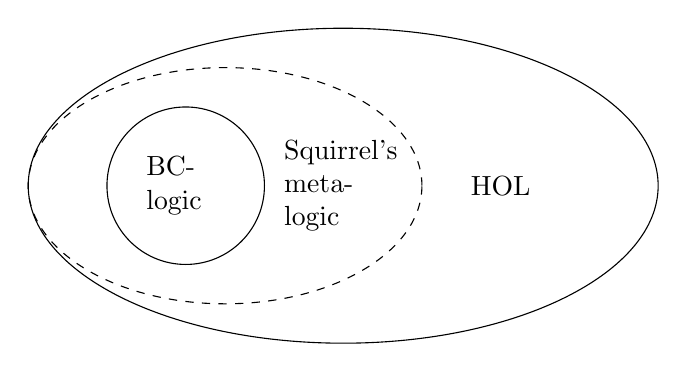
\begin{tikzpicture}
    \draw (0, 0) ellipse (4cm and 2cm);
    \draw[dashed] (-1.5, 0) ellipse (2.5cm and 1.5cm);
    \draw (-2, 0) circle (1 cm);

    \node at (2, 0) {HOL};
    \node[text width = 1.5cm] at (-0, 0) {Squirrel's meta-logic};
    \node[text width = 1cm] at (-2, 0) {BC-logic};
\end{tikzpicture}
\caption{Inheritance of HOL, BC-logic and Squirrel's meta-logic}\label{figure:1}
\end{figure}
\subsection{First Order Logic, High Order Logic and Metalogic}
To verify property of a computer program, logical systems like sequent calculus, natural deduction and Hilbert's system are applied. Most of these methods are based on first order logic(FOL), where proof goals are resolved stepwise by assumptions and axioms. On the basis of that, high order logic introduces type system, allowing for more flexible data types and more complicated proofs. Similarly, the proof systems can be extended to high order logic(HOL), which guarantees the theoretical background for proof assistants. \cite{logic1}

Though applying first order logic and high order logic, the proof assistants usually requires other systems, such as Zermelo-Fraenkel set theory. Additionally, we sometimes want to distinguish the user-level commands and automated proof processes, hence a different logical expression system is required, i.e. meta-logic. Meta-logic usually summarizes and integrates all available proof systems, and is used as the keywords or commands in the proof assistants. The basic logical terms, e.g. first order logic, can be converted to meta-logic terms, whereas a reverse conversion is sometimes not possible and less meaningful. \cite{Squirrel}

In this paper we study the ingenuity of BC-logic and its successor, the meta-logic of Squirrel. The inheritance between first order logic, BC-logic and meta-logic of Squirrel is given in \hyperref[figure:1]{Fig. 1.} Since Squirrel provides sufficient HOL components, there is no obvious boundary between Squirrel's meta-logic and HOL. BC-logic, however, focuses mostly on verification of ground instances. Hence we may see an obvious border between it and the meta-logic of Squirrel.

\subsection{Symbolic Model vs. Computational Model vs. CCSA}
\label{sec:back}
The Symbolic model and the computational model are the two most studied models of adversaries against cryptographic protocols, each has its own advantages and disadvantages. The symbolic model, or the Dolev-Yao model, models the protocol primitives as the blackboxes functions and thus defines a fixed set of behaviours of attackers, i.e. the attackers' behaviours are restricted under this framework.\cite{Dolev-Yao} However, in reality, the attacker are more mutable and less predictable, hence the symbolic models cannot cover all possible attacks even though it is suitable for formalisation and automated reasoning. The other kind of the models, the computational model, covers a larger range of attackers. It treats messages as bitstrings, which are easily printed and read on a tape. For this reason, the primitives and the attackers are assumed to be probablistic Turing machines. However, due to the complexity of Turing machines, this stronger model fails to provide an easy context for automated reasoning via a modern ITP. Both models, however, are limited to theoretical level, where attacks on the hardware devices are neglected. Due to their simplicity for modeling and automation, the symbolic models were overwhelmingly studied in the past two decades, hence more researchers now would like to explore the untouched domain of the computational models.\cite{SOK1}

In the paper by Baelde et al. 2020\cite{Squirrel}, a new type of model, Computational Complete Symbolic Attacker(\textbf{CCSA}) was introduced. It is built up from the BC-logic allowing for the proof automation for the computational models, too. In this model, an attacker can be any arbitrary function, that is verifiable in the ITP Squirrel, which is discussed and analyzed in following section \hyperref[sec:squirrel]{A Case study of the Squirrel Prover}. An overview of all three kinds of models mentioned is given in the \hyperref[figure:2]{Fig. 2.} An apparent inheritance relationship of three mentioned models can be easily witnessed, which corresponds to the sequence how researchers discovered and designed these three models.
\begin{figure}
\centering
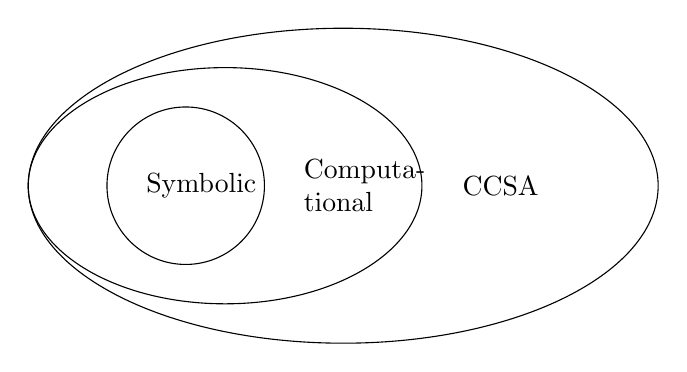
\begin{tikzpicture}
    \draw (0, 0) ellipse (4cm and 2cm);
    \draw(-1.5, 0) ellipse (2.5cm and 1.5cm);
    \draw (-2, 0) circle (1 cm);

    \node at (2, 0) {CCSA};
    \node[text width = 1cm] at (-0, 0) {Computa-tional};
    \node[text width = 1cm] at (-2, 0) {Symbolic};
\end{tikzpicture}
\caption{Inheritance of symbolic, computational and CCSA model}\label{figure:2}
\end{figure}
\subsection{Terminology}
\begin{itemize}
    \item Ground instance. In FOL, variables are either free or bounded by quantifiers, which includes the universal quantifier $\forall$ and the existential quantifier $\exists$. Instances of first order terms can be obtained by replacing bounded variables with suitable constants and removing the bounding quantifier. An instance where all bounded variables are replaced with constants and no free variable exists is called ground instance.\cite{logic2}
    \item Trie. A trie, or a prefix tree, is a type of k-nary search tree used for storing and locating strings with a specified prefix. It can be also viewed as a deterministic finite automaton without circles. Hence it is efficient for storing and searching messages when the transition rules are simple and straightforward.\cite{trie}
    \item Sequent calculus. First proposed by Gerhard Gentzen, sequent calculus is a style of formal logical argumentation in which every line of a proof is a conditional tautology instead of an unconditional tautology. It is written in a bottom-up big-step format, where proofs finally lead to a tautology. It also has variations like Hilbert's system and natural deduction, which are all widely used in the implementation of proof assistants.\cite{logic1}
    \item Proof tactics. Proofs tactics are commands in ITPs that build the proofs. Similar to manual proofs on paper, we can show a theorem/lemma by the definition of a term, by applying a proven theorem/lemma or by case distinction etc. Tactics of this sort are usually named as \textbf{apply}, \textbf{case} etc. To accelerate the process, a few proof approaches, e.g. variations of sequent calculi as mentioned, are implemented as tactics. This usually saves users a lot of time and spaces in generating the proofs. The naming convention of such tactics differs from developers. A tactics named \textbf{auto} is often supported. Some provers can also support user-defined tactics.\cite{LeanTactics}
\end{itemize}

\section{BC-Logic in an overview}
The general idea of the BC-logic is formalising the protocols and features of protocols as logical terms and checking the satisfiability of logical formulae. Apart from some trivial boolean property, the indistinguishability is more attractive to the researchers. An attacker should not be able to distinguish between two executions of a protocol, given a set of identical inputs and outputs. Practically, this means that an attacker should not be able to tell the difference between two functionally equivalent protocols.

To show that two or multiple protocols are computationally indistinguishable, we have to show that they behave negligibly differently when attacked by the same adversary. However, it is hard to prove this property if we want to show that the protocols have the same computation trace. The example given in \hyperref[example]{Fig. 2} consists of two functions that are functionally equivalent. Both of the functions return a random bit, when receiving a random integer by a parity check. On the one hand, the function \textit{f} has to be split into two computation traces due to the existence of the condition statement. One the other hand, then function \textit{g} has only one trace. Thus, they are considered distinguishable if we apply this traditional approach.
\begin{figure}
\begin{align}
    f\; x &:= if\; x\; mod\; 2 = 0\; then\; 0 \; else\; 1 \nonumber \\
    g\; x &:= x\; mod\; 2\nonumber
\end{align}
\caption{2 functionally equivalent functions}
\label{example}
\end{figure}

BC-logic provides an alternative---it folds the protocols. In most approaches that model a communication protocol, e.g. $\pi$-calculus, condition statements, loop or recursive features, communication between different channels and its control are necessary. Except for communication and control of multi-channels, all syntax components can be decided, allowing for choosing the suitable transition rule at each step when a ground instance is available. This technique, proposed by Bana and Comon, is referred to as folding the protocol, where all transition rules are mapped into a protocol tree. We fold the protocol tree in a top-down manner, where condition statements decide between branches, and concatenations extend the messages. In the end, only one transition rule should remain. This avoids splitting the trace as in the traditional approach. When a ground instance is given, the evaluation of the rules can be executed to derive the messages that are sent or received. On the basis of that, indistinguishability is defined with the predicate $\sim$, and can be thus used directly in logical formulae. Additionally, the same free function symbols are used to abstract all attackers in the same formulae. It is then possible to obtain a first order formula, which represents the protocols and property that we want. By checking the unsatisfiability of the formula, we can tell the inexistence of the potential attackers.

In the end, it is possible to show the computational indistinguishability of the protocols. This approach allows for verification of protocols under a computational model, excluding the necessity to consider the probablistic Turing machines, enabling the possibility to apply the computer-aided verification on the computational models, which was previously limited to the symbolic models. 

Two areas for further researches were left by Bana and Comon: the efficiency  and the usefulness of the BC-logic. We dived into both of the questions and came up with some results. \cite{BC-logic}

\section{Complexity of BC-Logic}
Bana and Comon proposed that the verification of BC-Logic can be executed in within a polynomial bound but did not gave formalisation and proof. We focused on this topic and verified the polynomial complexity with the ITP Isabelle. To show the complexity of certain functions, asymptotic classes are necessary. For convenience purposes, we do not show the theorem direct w.r.t. the definition, but choose to apply the following lemma alternatively.
\begin{align}
     \exists\textit{a b}. \textit{f}(\textit{n}) = \textit{a} \cdot \textit{n} + b \Longrightarrow \texit{f} \in \mathcal{O}(\textit{n}) \nonumber
\end{align}
Since our implementation covers only complexity class $\mathcal{O}(\textit{n})$, we do not give a generalized lemma on any arbitrary complexity classes. However, a formalized generalisation can be given in a recursive form.

To derive the complexity, we increase the metrics by one time unit per function call and operation. When evaluating the BC-Logic terms, we increase the metrics by one time unit per operator, i.e. constructors of the BC-Logic terms, with a few exceptions to be discussed in the next few subsection.
\subsection{Complexity of the evaluation of syntax}
The crucial work is verifying that the evaluation of BC-logic terms are executable within the polynomial-time. This is also the preparation for the second part, the verification of the folding process. For formalisation of BC-logic terms, we modelled two different types of variables, \textbf{msg} and \textbf{bool}. We support the syntax proposed by Bana and Comon, adding a few configuration for the purpose of automated reasoning.
Supported are the empty message(\textbf{EMPTY}), atomic message(\textbf{ATOM}), condition statement of \textit{if ... then ... else ...}(\textbf{ITE}) and concatenation of messages (\textbf{CONS}) for \textit{msg} type, and true(\textbf{T}), false(\textbf{F}), equality of two messasges(\textbf{EQ}) and equality of the length of two messages(\textbf{EQL}) for \textit{bl} type. Now that the \textbf{EQL} operator requires the comparison of the length of the \textbf{msg} and \textbf{bl}, we define a length function, \textbf{msg\_len} for \textbf{msg} and \textbf{bl\_len} for \textbf{bool}, in which all operators increase the length of message by one unit and atomic messages have the length of its original string.

Since both \textbf{msg} and \textbf{bool} require each other in their definition, mutually recursive functions and lemmata are required, which are fortunately supported by Isabelle. However, a proof of correctness and termination is necessary and can be mostly done by the automatic tactics. Moreover, we define the run-time functions, \textbf{T\_eval} for \textbf{msg} and \textbf{T\_bval} for \textbf{bool}, for evaluating both \textbf{msg} and \textbf{bool} recursively by increasing the result at each function call. A few examples for calculation of the evaluation of complexity are given in the table \hyperref[table:2]{2}. The corresponding commands in Isabelle are given in the  \hyperref[bcterms]{Fig. 4 and Fig. 5}
\begin{table}[ht]
\centering
\begin{tabular}{ ||p{3cm}|p{0.8cm}|p{3cm}|| }
     \hline
      Example in formulae & T\_eval & Evaluation Order\\
     \hline
     \rowcolor{gray!30}
     \textbf{if} ('msg'\textbf{==}'msg') \textbf{then} ('fst'\#'snd') \textbf{else} EMPTY & 15 & \textit{if...then...else} $\Rightarrow$ condition $\Rightarrow$ concatenation $\Rightarrow$ atomic strings \\
    'fst'\# (\textbf{if} ('msg'\textbf{$\sim\sim$}'msg') \textbf{then} 'snd' \textbf{else} 'thd') & 15 &
    concatenation $\Rightarrow$ atomic string $\Rightarrow$ \textit{if...then...else} $\Rightarrow$ condition $\Rightarrow$ atomic string\\
    \rowcolor{gray!30}
    'msg'=='msg' & 7 & equality $\Rightarrow$ atomic strings\\
    'msg'$\sim\sim$'msg' & 7 & length equality $\Rightarrow$ atomic strings\\
     \hline
\end{tabular}
\\[10pt]
\caption{examples of evaluation of time complexity}
\label{table:2}
\end{table}
\begin{figure}
\centering
   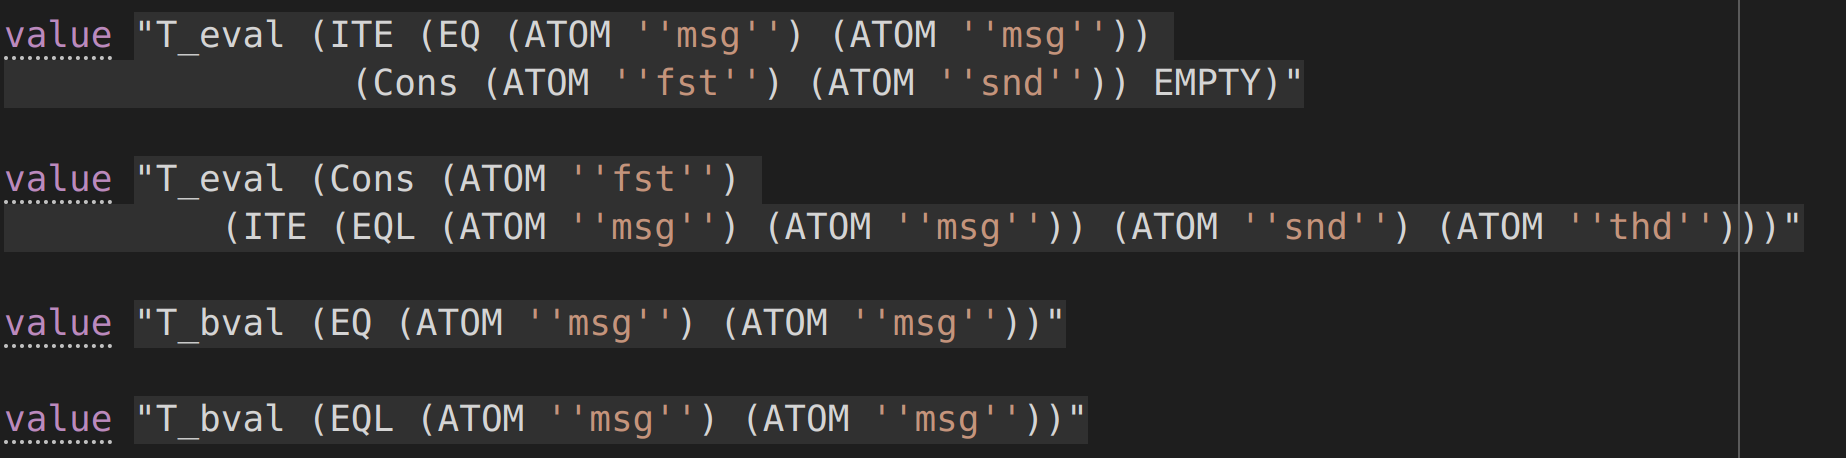
\includegraphics[width=0.5\textwidth]{Isabelle_command_1.png}
\caption{Examples of commands for evaluation of time complexity}\label{figure:3}
\end{figure}

Finally, we managed to show that the evaluation procedure of \textbf{msg} and \textbf{bl} can be completed within the linear time with regards to the length of the message.
\begin{figure}
\centering
\begin{align}
    \textit{msg} :=& \textbf{ EMPTY } | \textbf{ ITE } \textit{bl msg msg } \nonumber \\ 
    &| \textbf{ CONS } \textit{msg msg } | \textbf{ ATOM } \textit{string} \nonumber\\
    \textit{bl} :=& \textbf{ EQ } \textit{msg msg } | \textbf{ EQL } \textit{msg msg } | \textbf{ T } | \textbf{ F} \nonumber
 \end{align}
 \begin{align}
    &\textbf{T\_eval } \textit{msg} \leq \textbf{msg\_len } \textit{msg} \nonumber\\
    &\textbf{T\_bval } \textit{bl} \leq \textbf{bl\_len } \textit{bl} \nonumber\\
    & \exists \textit{a b}. \textbf{T\_eval } \textit{msg} \leq a \cdot (\textbf{msg\_len} \textit{ msg}) + b\nonumber\\
    & \exists \textit{a b}. \textbf{T\_bval } \textit{bl} \leq a \cdot (\textbf{bl\_len} \textit{ bl}) + b\nonumber
\end{align}
\caption{Definitions and theorems for the evaluation of BC-logic terms}
\label{bcterms}
\end{figure}
\subsection{Complexity of folding protocols}
The core of BC-logic is folding the protocols, it is the preparation for checking the unsatisfiability of the BC-logic term. All transition rules are folded into one single rule. While multiple rules are not easily formalised and verified by an ITP, the resulting single rule returns a BC-logic term that can be directly passed into logical formula. When a ground instance is available, the verification of this term is possible to be finished within the constant time. Hence we model a protocol into a trie\cite{trie}, where each transition rule is mapped to a node. An example of folding the protocol is given in \hyperref[figure:7]{Fig. 7}. A path to the leaf is summarized to be a message. 

There are two constructors for the \textit{proc\_trie} data structure, \textbf{Rt} and \textbf{Nd}, where \textbf{Rt} only occurs at the root of the trie and \textbf{Nd} implies an inner node. Each \textbf{Nd} stores \textbf{msg} and transition rules that start at this position in a list of pairs of \textbf{bool} and \textbf{proc\_trie}. When \textbf{bool} evaluates to true, the rule will be chosen and the \textbf{msg} in this branch will be concatenated to the current \textbf{Nd}. To preserve the property that the constructor \textbf{Rt} only exists at the root of the trie, we introduce an invariant function \textbf{valid} and its corelated helper functions as well as corresponding lemmata. With this function to ensure the invariant, we are able to show further property of the data structure.

It can be inferred that no leaf constructor is defined, whereas an empty list stands for a leaf. In addition, we did not model a trie using a conventional mapping but a list, hence some helper functions are necessary for showing the property of the data structure. \textbf{sz}, \textbf{lf} and \textbf{nd} count the nodes, leaves and inner nodes of the trie, whereas \textbf{get\_msg} returns the resulting message of the given ground instance when the transition procedure is over.
To show the correctness and use their property in formal proofs, the counting functions should fulfil the theorem that sum of the amount of the leaves and the amount of the inner nodes is equal to the amount of all nodes. All the definitions and required lemmas are given in the \hyperref[figure:9]{Fig. 9}

Now, the folding the protocol is folding the tree to a new tree which contains only one root and one inner node. All of the transition rules will be transformed into an \textit{if...then...else...} statement, where the we copy the boolean conditions and messages correspondingly to the condition and the \textit{then} branch of the statement, the \textit{else} branch is formed by transforming other rules at the same height. If the message is not a leaf in the tree, the process is executed recursively such that all the children nodes will be padded after the parent nodes. In this manner, all rules will be folded into one single message in the remaining rule. In this rule, \textit{root} is just an abstraction for the root of the tree, and \textit{true} means that the transition will always happen. Hence the resulting message can be directly used as a constant in the logical formulae. The folding result of the example in \hyperref[figure:7]{Fig. 7} is given in \hyperref[figure:8]{Fig. 8}.

It can be inferred that we use similar definition structure for \textbf{get\_msg} and \textbf{fold}, where the only difference is the choice between Isabelle syntax and BC-logic syntax. This corresponds exactly to the designing purpose of the folding protocol---folding allows for obtaining the message immediately, which brings part of the evaluation forward.

In the our proof, a mere induction is not sufficient, where we have to use the previously shown lemmata about the \textbf{valid} function to obtain the premises of our goal.
\begin{figure}
\centering
\begin{align}
      root, a &\xrightarrow{\theta_1} m_1, b\; &m_2, b \xrightarrow{\eta_1} n_1, c\nonumber\\
      root, a &\xrightarrow{\theta_2} m_2, b\; &m_3, b \xrightarrow{\eta_2} n_2, c\nonumber\\
      root, a &\xrightarrow{\theta_3} m_3, b \; &m_3, b \xrightarrow{\eta_3} n_3, c\nonumber
  \end{align}
\caption{A set of transition rules}
\end{figure}
\begin{figure}
\centering
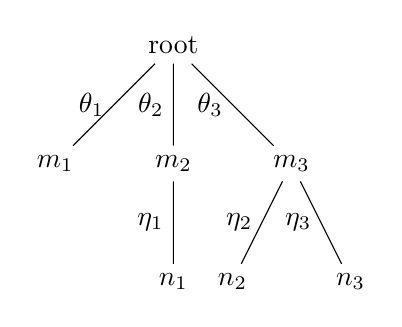
\begin{tikzpicture}
   \node{root}
     child {node {$m_1$} edge from parent node[left] {$\theta_1$}}
     child {node {$m_2$}
        child {node {$n_1$} edge from parent node[left] {$\eta_1$}} 
          edge from parent node[left] {$\theta_2$}}
     child {node {$m_3$}
        child {node {$n_2$} edge from parent node[left] {$\eta_2$}}
        child {node {$n_3$} edge from parent node[left] {$\eta_3$}} 
          edge from parent node[left] {$\theta_3$}};
\end{tikzpicture}
\caption{An equivalent protocol trie}\label{figure:7}
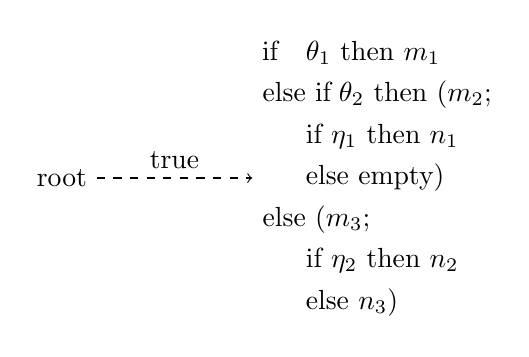
\begin{tikzpicture}
   \node (root) at (-4, 0) {root};
   \node[align=left] (dest) at (0, 0) {$\begin{aligned}
      \text{if}\quad& \theta_1 \text{ then } m_1 
      \\\text{else}&\text{ if}\; \theta_2 \text{ then (} m_2; 
      \\&\text{if }\eta_1\text{ then }n_1 
      \\&\text{else empty)} 
      \\\text{else}&\text{ (}m_3; 
      \\&\text{if }\eta_2\text{ then }n_2 
      \\&\text{else }n_3\text{)}
      \end{aligned}$};
    \path (root) edge[->, dashed] node[above] {true} (dest); 
\end{tikzpicture}
\caption{The result of folding this protocol trie}\label{figure:8}
\end{figure}
\begin{figure}
\centering
\begin{align}
    \textit{proc\_trie} :=& \textbf{ Rt } (\textit{bl} \times \textit{proc\_trie}) \textit{ list} \nonumber \\
            &| \textbf{ Nd } \textit{msg } (\textit{bl} \times \textit{proc\_trie}) \textit{ list}\nonumber\\
    \textbf{fun valid} ::& \textit{ proc\_trie } \Rightarrow \textit{ bool} \nonumber
\end{align}
\begin{align}
    &\textbf{valid } (\textbf{Rt } (\textit{x\#l})) \Longrightarrow \textbf{valid } (\textbf{snd } \textit{x}) \land \textbf{valid } (\textbf{Rt } \textit{l}) \nonumber\\
    &\textbf{valid } (\textbf{Nd } (\textit{x\#l})) \Longrightarrow \textbf{valid } (\textbf{snd } \textit{x}) \land \textbf{valid } (\textbf{Rt } \textit{l}) \nonumber
\end{align}
\begin{align}
    &\textbf{fun } \textbf{sz } := \textit{proc\_trie} \Rightarrow \textit{nat} \nonumber\\
    &\textbf{fun } \textbf{nd } := \textit{proc\_trie} \Rightarrow \textit{nat} \nonumber\\
    &\textbf{fun } \textbf{lf } := \textit{proc\_trie} \Rightarrow \textit{nat} \nonumber\\
    &\textbf{fun } \textbf{get\_msg} := \textit{proc\_trie} \Rightarrow \textit{msg} \nonumber
\end{align}
\begin{align}
    (\textbf{nd } \textit{proc\_trie}) + (\textbf{lf } \textit{proc\_trie}) = \textbf{sz } \textit{proc\_trie}\nonumber
\end{align}
\begin{align}
    &\textbf{fun } \textbf{fold } := \textit{proc\_trie} \Rightarrow \textit{msg}\nonumber\\
    &\textbf{fun } \textbf{T\_fold } := \textit{proc\_trie} \Rightarrow \textit{nat}\nonumber
\end{align}
\begin{align}
    &\textbf{eval } (\textbf{get\_msg } \textit{proc}) = \textbf{eval } (\textbf{fold } \textit{proc}) \nonumber\\
    &\textbf{valid } \textit{proc} \Longrightarrow \textbf{T\_fold } \textit{proc} \leq \textbf{sz } \textit{proc} + \textbf{nd } \textit{proc} \nonumber\\
    &\exists \textit{a b}. \textbf{valid } \textit{proc} \Longrightarrow \textbf{T\_fold } \textit{proc} \leq a \cdot (\textbf{sz } proc) + b \nonumber\label{eq: 8}
\end{align}
\caption{Definitions and theorems for folding the protocols}
\label{figure:9}
\end{figure}
We also showed that this procedure is completed within the linear time with regard to the size of the tree, i.e. the number of transition rules. 

Finally, we integrate the result of both evaluation and folding to obtain a general theorem about the complexity. This theorem is given in \hyperref[figure:10]{Fig. 10} Our implementation shows that the polynomial-time complexity proposed by Bana and Comon is correct, indicating that BC-logic is an efficient approach in term of verification of the computational model. \\
\begin{figure}
\centering
\begin{align}
    \textbf{fun eval\_proc} &:= \textit{proc\_trie} \Rightarrow \textit{string} \nonumber\\
    \textbf{fun T\_eval\_proc} &:= \textit{proc\_trie} \Rightarrow \textit{nat} \nonumber
\end{align}
\begin{align}
     \exists \textit{a1 a2 b}. \textbf{valid } \textit{proc} \Longrightarrow& \nonumber\\ 
     \textbf{T\_eval\_proc} \textit{ proc}  &\leq a1 \cdot (\textbf{sz } \textit{proc})\nonumber\\
     &+ a2 \cdot (\textbf{msg\_len } (\textbf{fold } \textit{proc})) + b\nonumber
\end{align}
\caption{The resulting correctness theorems}
\label{figure:10}
\end{figure}

\subsection{What our weakened implementation ignores}
Since our implementation only focused on the fundamental parts of BC-logic, there are a few things that we have ignored in either formalisation or proofs. We list them here and explain how they are not necessary in our weakened model.
\begin{itemize}
    \item Parallel channels. In the traditional $\pi$-calculus, a constructor that copies the current channel to create an identical channel is available. However, it was not discussed in the original paper of BC-logic, so we also ignored it in our studies.
    \item Boolean operators. We did not include Boolean operators, such as \textbf{AND}, \textbf{XOR}, etc. in our implementation. The verification of these Boolean operators only increases the complexity by one time unit for each occurrence, so ignorance of them does not raise a significant error, but decreases the complexity of the implementation. A future inclusion of them is expected.
    \item Configuration of the trie structures. We did not implement conventional functions that changes the data structure of our protocol trie, e.g. \textbf{insert} \textbf{delete} etc. Since protocols are a fixed set of transition rules, such functions are not necessary. However, the insertion function is useful to forge the protocol trie from the set of the transition rules. Hence it should be implemented and verified. This is also a direction for further and deeper research.
    \item Length of a message. In the original definition of messages in the computational model, they are a set of bitstrings, consisting of only \textbf{1} and \textbf{0}. In our implementation, we directly use the length of any arbitrary strings. This is acceptable, because the default encoding scheme in Isabelle ensures that all characters possess the same number of bits.
    \item Modeling of protocol participants, i.e. states in trie. In a tree-based data structure, there is not existent circles. In practice, it happens seldom in the context of protocols. A protocol subjects may send and receive messages multiple times, which may visit the same node multiple times and brings a circle. To avoid circles and loops in our trie, we use the same technique as applied in Bana and Comon's paper: Instead of modeling the protocol participants as an inner node, we use their internal states by giving every state a timestamp after send and receiving the messages. An internal state can not be repeated, hence no circle would exist in the trie. 
\end{itemize}
\section{Meta-logic of the Squirrel Prover}
\begin{table}[ht]
\centering
\begin{tabular}{ ||p{1.5cm}|p{6cm}|| }
     \hline
      Name & Supported constructions\\
     \hline
     \rowcolor{gray!30}
     Message initialisation & \textit{T :=} $\tau$ $\mid$ init $\mid$ a[$i_1$,...,$i_k$] $\mid$ pred(\textit{T}) \\
     Message configuration & \textit{t :=} \textit{x} $\mid$ n[$i_1$,...,$i_k$] $\mid$ f[$i_1$,...,$i_k$]($t_1$,...,$t_n$) $\mid$ input@\textit{T} $\mid$ output@\textit{T} $\mid$ frame@\textit{T} $\mid$ if $\phi$ then \textit{t} else \textit{t'} $\mid$
     find $\Vec{i}$ such that $\phi$ in \textit{t} else \textit{t'}\\
     \rowcolor{gray!30}
     Boolean predicates & \textit{A := } \textit{t} = \textit{t'} $\mid$ \textit{i} = \textit{i'} $\mid$ \textit{T} = \textit{T'} $\mid$ \textit{T} $\leq$ \textit{T'} $\mid$ cond@\textit{T} $\mid$ exec@\textit{T}\\
     First-order terms & \textit{$\phi$ := } \textit{A} $\mid$ $\top$ $\mid$ $\bot$ $\mid$ $\phi \land \phi'$ $\mid$ $\phi \lor \phi'$ 
     $\mid$ $\phi \Rightarrow \phi'$ $\mid$ $\neg \phi$ $\mid$ $\forall i. \phi$ $\mid$ $\exists i. \phi$ $\mid$ $\forall \tau. \phi$ $\mid$ $\forall \tau. \phi$ \\
     \hline
\end{tabular}
\\[10pt]
\caption{List of meta-logic terms and formulae in Squirrel.}
\label{table:3}
\end{table}
In comparison to basic BC-logic terms, the Squirrel Prover introduces a different logical systems, which supports the operations proposed in BC-logic as well as further first order and communication components, enabling more complicated construction of protocols.  In total, there are three possible types of meta-logic terms:
\begin{enumerate}
    \item terms of the type \textit{message} are bitstrings of messages exchange between entities of the protocol.
    \item terms of the type \textit{timestamp} trace the time points during the execution process of the protocol. 
    \item terms of the type \textit{index} serves for the usage of identification of the unbounded collections of entities in the protocol and execution process.
\end{enumerate}
A detailed summary of meta-terms and meta-formulae is given in Table \hyperref[table:3]{3}.\\
Additionally, sequent calculi are introduced to represent rules used by the prover. Several basic rules as well as a few collary rules were given by Baelde et al. On the basis of that, it is also possible to generate further admissible rules. However, in the actual implementation of the proof assistant, such behaviour is avoided, where users can alternatively generate self-defined lemmata to support their proofs. We checked the practical usage of the Squirrel by performing a case study in a few chosen examples with the help of the summarized knowledge.

\section{A case study of the Squirrel Prover}
\label{sec:squirrel}
\subsection{An overview of the Squirrel Prover}
The Squirrel Prover is a proof assistant for protocols. It is based on first-order logic and provides guarantees in the computational model. The programming language on which Squirrel is built is Ocaml. It supports an executable which is callable over the terminal by passing the proof scripts with the extension name \textit{.sp}. This is an automation mode, where all proofs are analysed immediately. Additionally, an emacs tool via Proof General\cite{ProofGeneral} is also available, in which the users can interact with the proof assistant and control the stepwise proof on their  own. Similar to most interactive theorem provers, Squirrel offers a few basic tactics for users to proof their theorems, which are also usable for later proofs. An overview of proof tactics available in Squirrel is given in \hyperref[table:4]{Table 4}. The Squirrel prover also provides a limited stepwise proof using the keyword \textbf{have}, which enables a more complex proof structure. However, due to its late occurrence, there is up till now neither official proof library nor automated proof search tools available, making up a larger room for development and improvement.
\begin{table}
\begin{tabular}{ ||p{1.5cm}|p{6cm}|| }
     \hline
      Tactic Name & Explanation\\
     \hline
     \rowcolor{gray!30}
     \textbf{intro} & fixing variables of universal quantifiers and obtaining the premises in the goal\\
     \textbf{split} & splitting the premises that are combined with the logical \textbf{AND}\\
     \rowcolor{gray!30}
     \textbf{apply} & applying a rule or a known fact to the goal\\
     \textbf{rewrite} & rewriting the goal or the given rule with the given equality\\
     \rowcolor{gray!30}
     \textbf{left, right} & choosing to branch in a goal combined by a logical \textbf{OR}\\
     \textbf{case} & case distinction on the given term\\
     \rowcolor{gray!30}
     \textbf{fresh} & showing that the probability of equality of 2 different variables is negligible\\
     \textbf{refl} & \textit{contrart to \textbf{fresh}}, a variable is equal to itself\\
     \rowcolor{gray!30}
     \textbf{auto} & an integration of several rules for faster automation\\
     \textbf{fa} & function application of the equal terms should be equal\\
     \rowcolor{gray!30}
     \textbf{collision} & collision detection in the hash functions\\
     \textbf{euf} & unforgeability of the hash functions, must be invoke on \textit{h(v, k) = u}\\
     \rowcolor{gray!30}
     \textbf{prf} & replacing a hashing statement with an \textit{if...then...else} statement\\
     \textbf{depends} & Fact inference by evaluating the order of events\\
     \hline
\end{tabular}
\label{table:4}
\\[10pt]
\caption{List of proof tactics in Squirrel.}
\end{table}

\subsection{An automated proof applying the Squirrel prover}
In our case study, we applied the Squirrel prover into practical usage. We firstly looked into the tutorial and previous examples  provided by the developers. Then we introduced the commonly used protocol, Kerberos, in modern networks. The work was however not finished, whose reasons are also covered in the next few chapter.
\begin{itemize}
    \item Tutorial provided by the developers. The tutorial starts with a few examples in basic logical operations. Fundamental mechanisms of security, such as hashing, key authentication etc., followed with a more difficult provability. Among the tactics given in \hyperref[table:4]{Table 4}, \textbf{euf} and \textbf{prf} are assumptions especially needed for security property. Thus, they are rather more important when we want to show a cryptographic or secure property. The other logic-based tactics are less important, but they are still widely used to show the formalized logical property of our protocols.
    \item Examples provided by developers. On the basis of the tutorial, the developers verified a few more
    features of a group of selected protocols. This includes signed Decisional Diffie-Hellman asumption, SSH with forwarding agent etc. All the tutorials and examples were nicely proven and commented, allowing for starters to have a better understanding. However, a documentary manual or multi-media sources for tutorial is still missing due to the current early-stage version of the tool.
    \item Our exploration: Key Distribution Center. Short for KDC, the key distribution center is a key authentication model, in which a server generates a one-time key for each communication trial. This procedure ensures the secure communication between clients. However, this protocol requires a trusted third party, otherwise a man-in-the-middle attack is possible. A famous protocol that applies this model is Kerberos.\cite{Kerberos} \\
    Unfortunately, we failed to finish the formalisation and verification of this protocol. The main reason for it is the lack of knowledge and experiences in protocol verification. Additionally, the design of timestamps in Squirrel is also a bit hard to understand and deal with for starters, which is a potential improvement of the tool. 
\end{itemize}
In conclusion, the Squirrel prover is capable of showing a number of features of modern communication protocols. However, the tool itself is still in its growth. Thus, the automation of the proof is not optimal, and the environment is not easy for starters. Starters in formal verification and/or formal methods in security are suggested to begin with other tools as listed in \hyperref[table:1]{Table 1} for better support and experiences.

\section{Evaluation}
\subsection{Complexity Analysis}
Since our defined trie is a functional data structure, we apply the conventional complexity analysis that every function call and operation adds up one unit to the result. This is a widely used approach, first introduced by D. Knuth et al. in the book \textit{Art of Computer Programming}.\cite{ART} In the specified case of Isabelle, we use the techniques proposed by T. Nipkow et al. in the book \textit{Functional Algorithms, Verified!}. \cite{FAV} \hyperref[figure:11]{Fig. 11} gives the command in Isabelle to fold the example in the \hyperref[figure:7]{Fig. 7} and its result. It is noticed that the result is slightly different from what is expected, this is because of the implementation convenience that all messages now end with an \textit{if...then...else...} condition statement. However, the structures are syntactically equivalent and do not raise a significant complexity increase.
\begin{figure}
\centering
   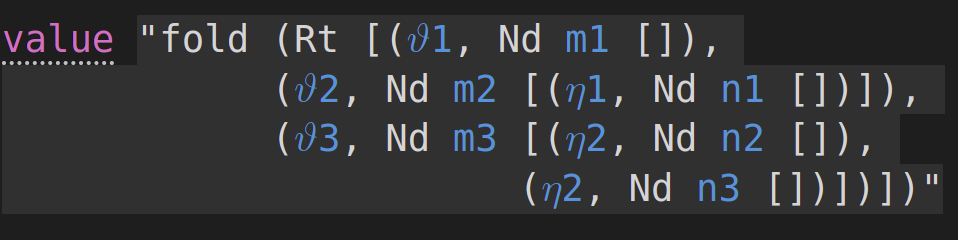
\includegraphics[width=0.4\textwidth]{Isabelle_command.png}
   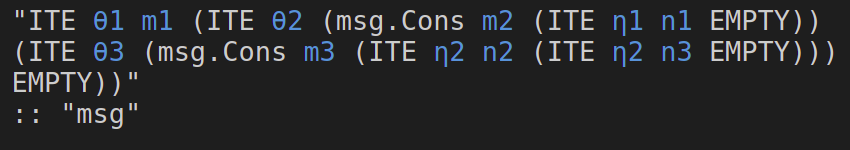
\includegraphics[width=0.4\textwidth]{Isabelle_output.png}
\caption{Command and output of the Isabelle when folding the Example in \hyperref[figure:11]{Fig. 7}}
\label{figure:11}
\end{figure}
\subsection{Case study of Squirrel}
Provided that the Squirrel prover is sound and complete for the attackers under the \textit{CCSA} model, it is guaranteed that our case study over the given cryptographic schemes is correct. However, this is also limited to the \textit{CCSA} model. Should there be an attacker that cannot be modeled by BC-logic, our proof as well as the meta-logic of the Squirrel would not be guaranteed to be sound and complete any more.

Since cryptography is never ensured not to be vulnerable to any attackers, there might be in the future sorts of attackers that overcome the BC-logic. In that time a new model or extension of the current work are needed.
\section{Discussion}
\subsection{Complexity Analysis}
As shown in our ignorance during complexity analysis, we only did a complexity analysis on a weakened model of the BC-logic, showing that such verification of polynomial-time complexity is possible. A deeper and more comprehensive formalisation and proof is expected.

Since BC-logic was still on the theoretical level, our complexity analysis is sufficient. When it comes to actually implementation like Squirrel, our implementation should be extended in accordance to Squirrel's meta-logic. In practice, a theoretical analysis is less than enough, for that run time of practical software and hardware are more complicated that our theoretical estimation. Therefore, bench-marking for Squirrel is in the long term necessary and foreseeable, in order to evaluate the run time of the software better.
\subsection{Case study of Squirrel}
From the case study and original paper, we know that Squirrel is powerful in showing some cryptographic features of not only protocols but also attackers. However, it is still in its testing version, i.e. not officially published. Thus, more features of the prover as well as a larger proof library is to be expected in the future. 

With the occurrence and implementation of quantum computers, the traditional cryptographic schemes are under doubt whether they are still secure. In the meantime, cryptographic schemes designed especially for quantum computers also became a new topic in cryptograhy and IT-security. In 2022, a new post-quantum scheme for protocol verification was also designed for Squirrel.\cite{PostQuantum} It introduced a new direction for the studies on BC-logic and the Squirrel prover, which is a promising and wide field to dive in.

\subsection{Relation of our two parts of work}
In addition to the outlook of BC-logic and the Squirrel prover, we present an overview of how our two parts of work are integrated in term of implementation. We can divide the implementation of an interactive theorem prover into 3 levels. They are in the bottom-up order the foundation level, the integration level, and the user-interactive level. The foundation level consists of a theoretical proof system, e.g. \textbf{HOL} for \textbf{Isabelle} and \textbf{BC-logic} for \textbf{Squirrel} , and a programming language on whose basis the interactive prover is implemented, e.g. \textbf{c++} for \textbf{lean} and \textbf{Ocaml} for \textbf{Squirrel}. On this level, some basic operations are implemented. No interaction or proof from the user side is possible. On the integration level, some of the basic operations of the prover, along with the original programming language, are used to form the basic theory and proof system of the prover. The last level, the user-interactive level, is where users can interact with the prover and generate their own proofs. Some advanced libraries are in this level, even though they are important constitutions of the prover. Additionally, most main-stream provers also allow users to contribute to the open library, so that the community is vivid and growing.\cite{AFP}\cite{CoqComm}\cite{LeanContri}

In the first part of the work, we focused on the BC-logic and its complexity. It is the theory and proof system ascribed to the foundation level. In the second part, we studied the meta-logic of the Squirrel prover. This belongs to both the foundation and integration level. Lastly, we performed a case study on the Squirrel prover, proving the soundness of several well-known protocols, which is in the user-interactive level. It can be inferred that there is no direct relationship between the BC-logic and interactive proofs using Squirrel, just as no direction relation between the foundation level and user-interactive level. Meta-logic, however, integrates the two parts, just as how integration level integrates the two other levels. An accurate graphical description of this relationship is given in the \hyperref[figure:12]{Fig. 12}
\begin{figure}
\centering
   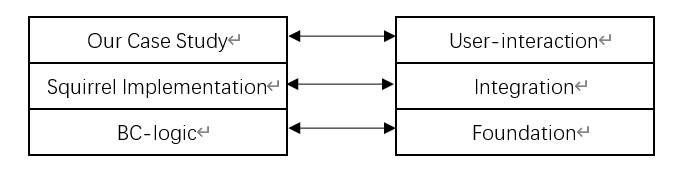
\includegraphics[width=0.5\textwidth]{ITP.png}
\caption{Structure of an ITP}
\label{figure:12}
\end{figure}

\section{Related Works}
Our work is mainly based on Bana and Comon's work\cite{BC-logic} in 2014 with a few studies into the 2021 paper by Baelde et al.\cite{Squirrel} Bana and Comon first introduced the \textit{CCSA} in 2012 \cite{CCSA} and then formalized a verification method, i.e. BC-logic in 2014. In 2016, Bana et al. analyzed the FOO electronic voting protocol in the provable security model using the technique of \textit{CCSA}.\cite{BanaVoting} Later, Bana et al. also introduced a verification method based on indistinguishability in 2019.\cite{CCSAVerif} This was also revealed in the Squirrel prover that followed later in 2021. There were also some researches that either applied or related to the BC-logic, but failed to provide more theoretical or technical improvements.

In the 2014 paper, two open questions were left unsolved---the complexity of verification and the usefulness of BC-logic. All the mentioned paper focused on the latter question, where researchers tried to develop better methods for the verification. Though not stated explicitly, the complexity was still considered when an actual tool was being developed. However, Baelde et al. pointed out that their prover only guarantees an asymptotic security bounds rather than complex security bounds, hence the real performance and complexity should be considered by the users. In 2022, Cremers et al. extended the existing Squirrel prover to support post-quantum cryptographic schemes. This also extends the usefullness and the compleixty analysis to the post-quantum cryptography.\cite{PostQuantum}

We performed a complexity analysis on the theoretical BC-logic with a few limitations. The work is new, for no one tried to formalize the complexity of BC-logic using an interactive theorem prover. Additionally, we introduced tries, i.e. prefix trees, to finish the formalisation. The modelling of protocols as trees was introduced by Bana and Comon, but the choice of tries and implementation in the prover Isabelle was promising and effective. We also dived into the relatively new prover based on BC-logic, giving some feedback that is helpful for new users to start with.

\section{Conclusion}
We have proved the polynomial bounds of evaluation and folding of a simplified and limited version of BC-logic with the help of the interactive theorem prover Isabelle. We also performed a case study on the interactive theorem prover Squirrel built on the basis of BC-logic. We managed to partially answer the 2 questions thrown by Bana and Comon in the 2014 paper\cite{BC-logic} that the verification of BC-logic can be efficiently done within polynomial time and it can be useful in practice. A brief overview of our finished work in Isabelle is given the github repository \url{https://github.com/AlexiosFan/Seminar_BC_Logic.git}. The failed trials in Squirrel were excluded.

As future work, extending the syntax of our simplified version of BC-logic to support more operations, such as logical \textbf{AND}, logical \textbf{XOR} etc, as well as defining a more comprehensive protocol trie, which allows operations like insertion and deletion, is planned. Furthermore, contribution to the Squirrel prover is also expected, as the tool and community are still growing.

\begin{thebibliography}{00}
\bibitem{BC-logic} Bana, Gergei, and Hubert Comon-Lundh. "A computationally complete symbolic attacker for equivalence properties." Proceedings of the 2014 ACM SIGSAC Conference on Computer and Communications Security. 2014.
\bibitem{Squirrel} D. Baelde, S. Delaune, C. Jacomme, A. Koutsos and S. Moreau, "An Interactive Prover for Protocol Verification in the Computational Model," 2021 IEEE Symposium on Security and Privacy (SP), 2021, pp. 537-554, doi: 10.1109/SP40001.2021.00078.
\bibitem{BanaVoting} Bana, G., Chadha, R., \& Eeralla, A. K. (2018, August). Formal analysis of vote privacy using computationally complete symbolic attacker. In Computer Security: 23rd European Symposium on Research in Computer Security, ESORICS 2018, Barcelona, Spain, September 3-7, 2018, Proceedings, Part II (pp. 350-372). Cham: Springer International Publishing.
\bibitem{Dolev-Yao} D. Dolev and A. Yao, "On the security of public key protocols," in IEEE Transactions on Information Theory, vol. 29, no. 2, pp. 198-208, March 1983, doi: 10.1109/TIT.1983.1056650.
\bibitem{pi-calculus} Milner, Robin. Communicating and mobile systems: the pi calculus. Cambridge university press, 1999.
\bibitem{Tamarin} Meier, Simon, et al. "The TAMARIN prover for the symbolic analysis of security protocols." International conference on computer aided verification. Springer, Berlin, Heidelberg, 2013.
\bibitem{ProVerif} Blanchet, Bruno. "Automatic verification of security protocols in the symbolic model: The verifier proverif." Foundations of security analysis and design VII. Springer, Cham, 2013. 54-87.
\bibitem{Coq} Huet, Gérard, Gilles Kahn, and Christine Paulin-Mohring. "The coq proof assistant a tutorial." Rapport Technique 178 (1997).
\bibitem{Isabelle} Nipkow, Tobias, Markus Wenzel, and Lawrence C. Paulson, eds. Isabelle/HOL: a proof assistant for higher-order logic. Berlin, Heidelberg: Springer Berlin Heidelberg, 2002.
\bibitem{LEGO} Luo, Zhaohui, and Robert Pollack. LEGO proof development system: User's manual. LFCS, Department of Computer Science, University of Edinburgh, 1992.
\bibitem{ProofGeneral} Aspinall, David. "Proof General: A generic tool for proof development." International Conference on Tools and Algorithms for the Construction and Analysis of Systems. Springer, Berlin, Heidelberg, 2000.
\bibitem{logic1} Troelstra, Anne Sjerp, and Helmut Schwichtenberg. Basic proof theory. No. 43. Cambridge University Press, 2000.
\bibitem{logic2} Schöning, Uwe. Logic for computer scientists. Springer Science \& Business Media, 2008.
\bibitem{trie} Knuth, Donald. "6.3: Digital Searching". The Art of Computer Programming Volume 3: Sorting and Searching (2nd ed.). Addison-Wesley. 1997. p. 492. ISBN 0-201-89685-0.
\bibitem{SOK1} Blanchet, Bruno. "Security protocol verification: Symbolic and computational models." International Conference on Principles of Security and Trust. Springer, Berlin, Heidelberg, 2012.
\bibitem{SOK2} M. Barbosa et al., "SoK: Computer-Aided Cryptography," 2021 IEEE Symposium on Security and Privacy (SP), 2021, pp. 777-795, doi: 10.1109/SP40001.2021.00008.
\bibitem{SOK/PA} Geuvers, Herman. "Proof assistants: History, ideas and future." Sadhana 34.1 (2009): 3-25.
\bibitem{Kerberos} Steiner, Jennifer G., B. Clifford Neuman, and Jeffrey I. Schiller. "Kerberos: An Authentication Service for Open Network Systems." Usenix Winter. 1988.
\bibitem{PostQuantum} Cremers, Cas, Caroline Fontaine, and Charlie Jacomme. "A Logic and an Interactive Prover for the Computational Post-Quantum Security of Protocols." S\&P 2022-43rd IEEE Symposium on Security and Privacy. 2022.
\bibitem{CCSA} Bana G, Comon-Lundh H. Towards unconditional soundness: Computationally complete symbolic attacker[C]//International Conference on Principles of Security and Trust. Springer, Berlin, Heidelberg, 2012: 189-208.
\bibitem{CCSAVerif} Bana G, Chadha R, Eeralla A K, et al. Verification methods for the computationally complete symbolic attacker based on indistinguishability[J]. ACM Transactions on Computational Logic (TOCL), 2019, 21(1): 1-44.
\bibitem{ART} Donald E K. The art of computer programming[J]. Sorting and searching, 1999, 3: 426-458.
\bibitem{FAV} Nipkow T, Blanchette J, Eberl M, et al. Functional Algorithms, Verified[J]. 2021.
\bibitem{AFP} https://www.isa-afp.org/
\bibitem{CoqComm} https://coq-community.org/
\bibitem{LeanContri} https://leanprover-community.github.io/contribute/index.html
\bibitem{LeanTactics} https://leanprover.github.io/theorem\_proving\_in\_lean/tactics.html
\end{thebibliography}
\end{document}

